\section{Methodology}

In this study, we use the SDO/AIA data of the Sun for three particular CME events (\cref{sec:selection_of_events}). These events are associated with special features like coronal dimming, filament eruptions and GLE event. The DEM for each image of the three events is obtained using the RML method. Next, we convert the full disk image of Sun to a point source (hereafter referred to as \textbf{Pointification}) and then inspecting if the signatures of the CMEs exist after the conversion and is similar to what is was before the conversion. Pointifying the Sun roughly translates to converting Sun to a star, or placing Sun to a place that's distant from Earth/observer in comparison to the distance between us and the Sun (defined as astronomical unit (1 AU $\approx 1.496\times10^{8}$ km)) such that it appears as a point source. We then analyse and compare the irradiance from the point source Sun and the full disk Sun using DEM to see if they show similar signatures of CMEs. Typically, Sun-as-a-star analysis involves selecting a region of interest on the surface of the Sun, making the assumption that this is the only region that affects the event under study, and that there is no activity anywhere on the rest of the Sun's surface, and then integrating the parameter of interest over the entire Solar disk. This is again a rough approximation to an actual star. Coronal dimming associated event is investigated to find the temperature range that shows the maximum amount of dimming.\\

In the following section, we discuss about the analysis tools used (\cref{sec:data_analysis_tools_used}), selection of events (\cref{sec:selection_of_events}), data used for the study (\cref{sec:data_used}), data pre-preprocessing (\cref{sec:data_pre_processing}) and data analysis procedure (\cref{sec:data_analysis_procedure}).

  \subsection{Data Analysis tools used}
  \label{sec:data_analysis_tools_used}

We have made use of Python programming language for our analysis. We have made extensive use of the following libraries: Numpy, Scipy, Aiapy, Sunpy, Pandas, Matplotlib, Astropy, Natsort, Multiprocessing, Datetime, Moviepy. In addition, we have used the RML method code for DEM analysis, as mentioned in \citep{Massa2023}. We have made use of SSW IDL for obtaining the temperature response curves for AIA. For visual inspection of the CME events, we have used JHelioViewer software. For quick inspection of the FITS file data, we have used FITSExplorer \footnote{link to the github repo: \url{https://github.com/dheerajshenoy/FITSExplorer}}, a software created as a side project by D. V. Shenoy.

\subsection{Event Selection}
\label{sec:selection_of_events}

We have chosen three CME events that have erupted on 2011 August 04, 2012 August 31 and 2021 October 28. The Solar and Heliospheric Observatory's  (SOHO) Large Angle and Spectrometric Coronagraph Experiment (LASCO) C2 (SOHO/LASCO) images of the CMEs obtained from the SOHO/LASCO CME catalog (\url{https://cdaw.gsfc.nasa.gov/CME_list/}) are given in \cref{fig:cme_events_soho_pics} and \cref{fig:cme_events_soho_pics_aia193}. Brief description of the events is given below:\\

\begin{enumerate}

        \item\textbf{2011 August 04}: This event has been refered from \citep{Mason2016} in which it is the \nth{20} Event. The event started at around 04:12 UT. This event occured from the source location N19W36 associated with the active region AR 11261.

        \item\textbf{2012 August 31}: This CME event was associated with a long filament eruption and it erupted around 19:49 UT. The CME associated with the filament travelled at over 900 miles per second.

    \begin{figure}[ht]
        \centering
        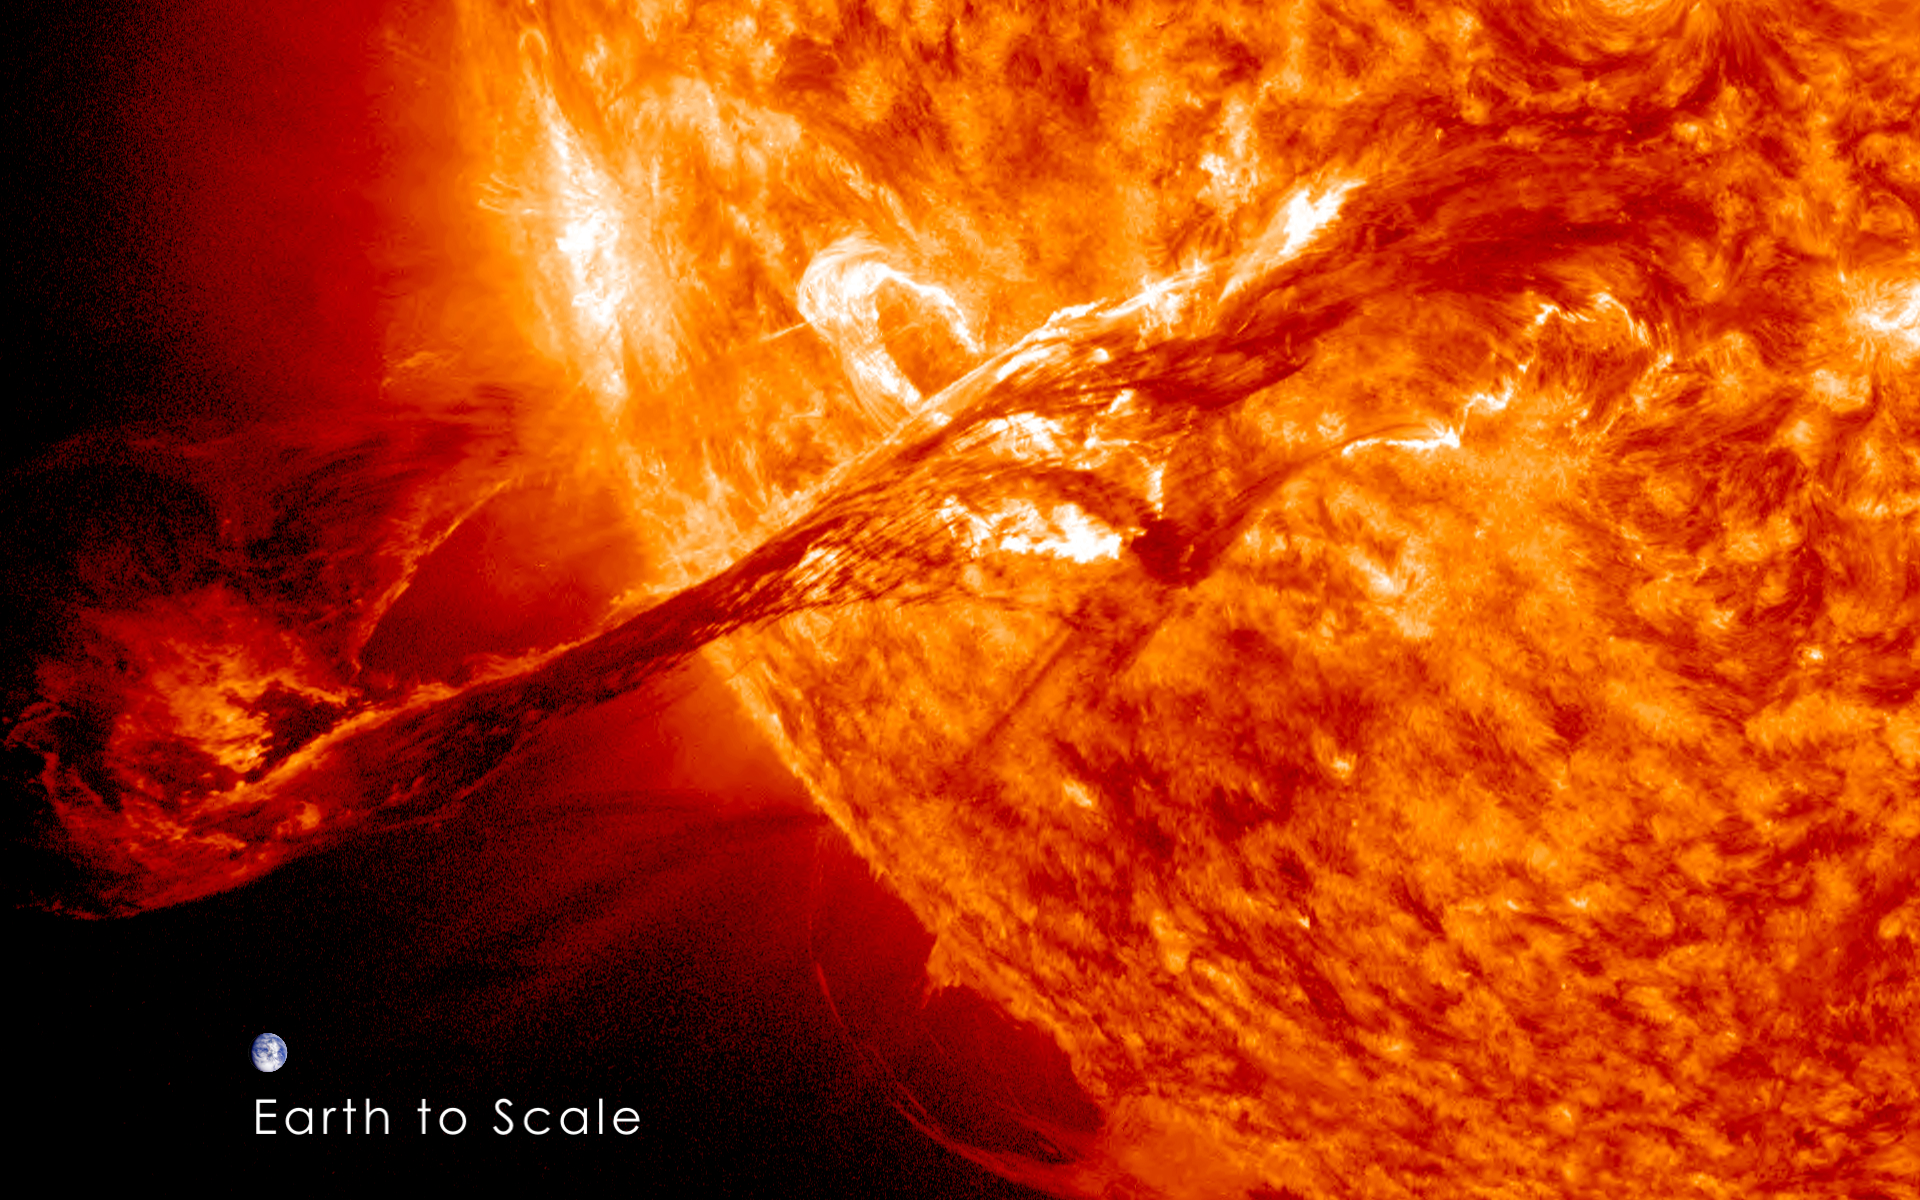
\includegraphics[width=0.5\textwidth]{images/aug_31_2012_event_sun_earth_image.jpg}
        \caption[Image of the Earth to scale of the 2012 August]{Image of the Earth to scale with the filament eruption of \nth{31} August 2012. Image credit: \url{https://svs.gsfc.nasa.gov/11095}}
        \label{fig:sun_earth_aug_31_2012}
    \end{figure}

        \item\textbf{2021 October 28}: This is an example for rarely occuring `ground level enhancement' event. During such an event, particles from the Sun are energetic enough to pass through the magnetic sheath that surrounds Earth and protects us from low energy solar outbursts. This was only the 73rd ground level enhancement since records began in the 1940s, and none have been recorded since \citep{Klein2022}. The event occured around 15:17 UT. The flare associated with the CME was an X1.1 class flare originated from the active region AR 2887.\\

\end{enumerate}

\begin{figure}[h!]
    \begin{subfigure}[b]{0.3\textwidth}
        \centering
        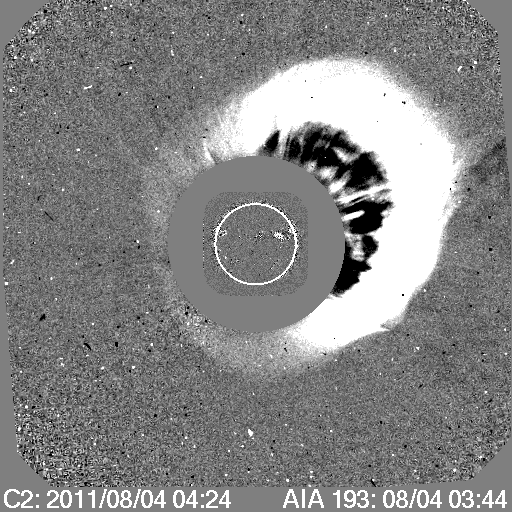
\includegraphics[width=\textwidth]{images/soho_cme_aug_04_2011.png}
        \caption[August \nth{4} 2011 CME]{August \nth{4} 2011}
        \label{fig:soho_cme_aug_04_2011}
    \end{subfigure}
    \hfill
    \begin{subfigure}[b]{0.3\textwidth}
        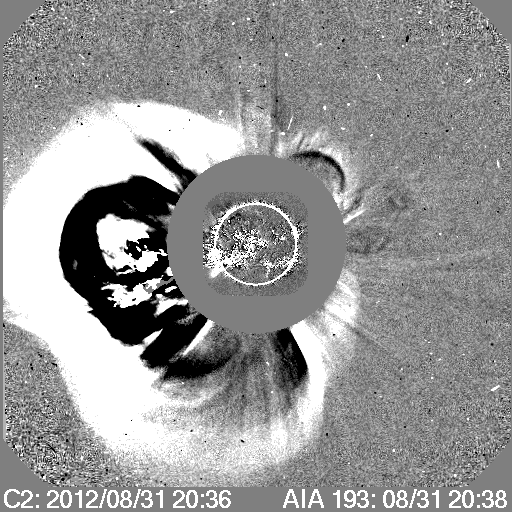
\includegraphics[width=\textwidth]{images/soho_cme_aug_31_2012.png}
        \caption[August \nth{31} 2012 CME]{August \nth{31} 2012}
        \label{fig:soho_cme_aug_31_2012}
    \end{subfigure}
    \hfill
    \begin{subfigure}[b]{0.3\textwidth}
        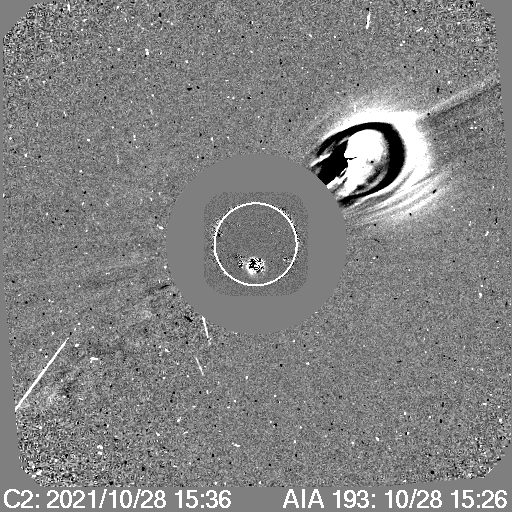
\includegraphics[width=\textwidth]{images/soho_cme_oct_28_2021.png}
        \caption[October \nth{28} 2021]{October \nth{28} 2021}
        \label{fig:soho_cme_oct_28_2021}
    \end{subfigure}
    \caption[SOHO/LASCO C2 running difference images of the selected events]{SOHO/LASCO C2 running difference images of the three selected events}
    \label{fig:cme_events_soho_pics}
\end{figure}

\begin{figure}[h!]
    \begin{subfigure}[b]{0.3\textwidth}
        \centering
        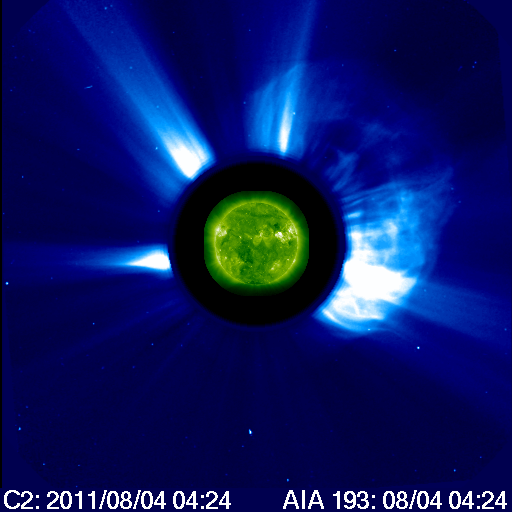
\includegraphics[width=\textwidth]{images/soho_cme_aug_04_2011_aia193.png}
        \caption[August \nth{4} 2011 CME]{August \nth{4} 2011}
        \label{fig:soho_cme_aug_04_2011}
    \end{subfigure}
    \hfill
    \begin{subfigure}[b]{0.3\textwidth}
        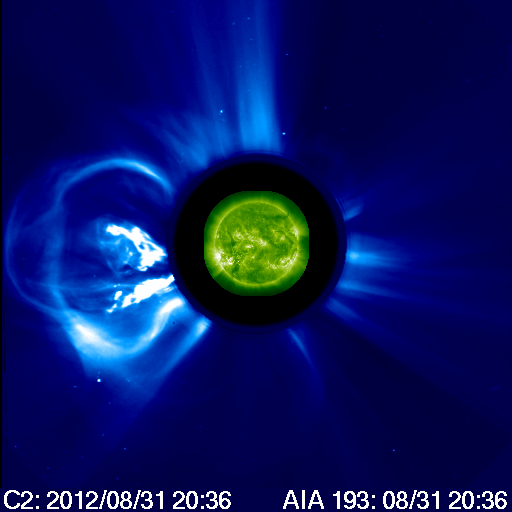
\includegraphics[width=\textwidth]{images/soho_cme_aug_31_2012_aia193.png}
        \caption[August \nth{31} 2012 CME]{August \nth{31} 2012}
        \label{fig:soho_cme_aug_31_2012}
    \end{subfigure}
    \hfill
    \begin{subfigure}[b]{0.3\textwidth}
        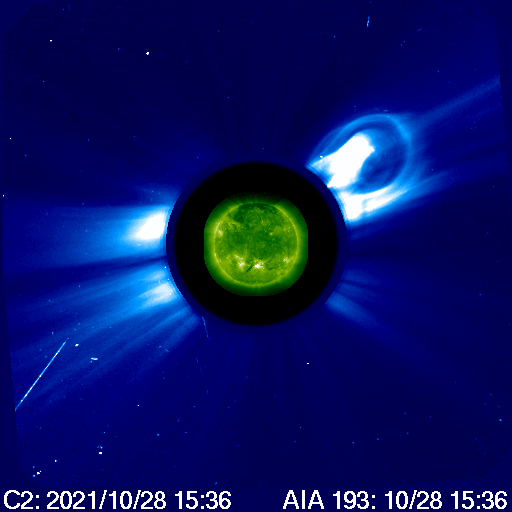
\includegraphics[width=\textwidth]{images/soho_cme_oct_28_2021_aia193.png}
        \caption[October \nth{28} 2021]{October \nth{28} 2021}
        \label{fig:soho_cme_oct_28_2021}
    \end{subfigure}
    \caption[SOHO/LASCO C2 images with AIA 193 \AA filter]{SOHO/LASCO C2 AIA 193 \AA\ filter images of the three selected events}
    \label{fig:cme_events_soho_pics_aia193}
\end{figure}

\subsection{Data}
\label{sec:data_used}

The SDO/AIA data is accessed through the JSOC portal (\url{http://jsoc.stanford.edu}) and required event data is obtained through the service. Event data consists of FITS files of Sun's image for the selected wavelength bands. For our analysis, we have used 5 channels: 94 $\AA$, 131 $\AA$, 171 $\AA$, 193 $\AA$ and 211 $\AA$. The remaining channels probe the Sun's surface temperature that is greater than what is required for our analysis. Also, the 335 $\AA$ channel has been excluded because of it's relatively weak temperature response at any temperature which affects the RML method used for the DEM analysis \citep{Massa2023}. We have used 10 hours of data for the \nth{4} August 2011 and \nth{31} August 2012 events, and about 7 hours of data for the \nth{28} October 2021 event. All three event data are at 2 minute cadence (Cadence refers to the frequency or timing of observations or measurements taken of the Sun or solar phenomena. It represents how often data is collected over a period of time).

\subsection{Image Pre-Processing}
\label{sec:data_pre_processing}

The downloaded FITS data files are 4096 $\times$ 4096 pixels in dimension. Data downloaded from the portal is level 1, which has been flat-fielded and processed to remove bad pixels and spikes (only for EUV channels), but not registered to preserve precise pixel values. As different channels of AIA have different roll angles, multi-wavelength analysis of any kind with level 1.0 data is problematic. Also, the pointing information contained in the headers of these FITS images will not be accurate, as it would have undergone changes compared to the information stored when the image was created. As mentioned in the SDO Data Analysis Guide, we have to use \texttt{aia\_prep.pro} function in Solar Software (SSW) IDL to correct or prepare the data used. Additionally, the images are downscaled from their original 4096 $\times$ 4096 pixel dimension to 512 $\times$ 512 pixels using sunpy as obtaining DEM solutions for the 4k dimension would be really time consuming and unnecessary as we are comparing full disk and point source DEM solutions.\\

The \textbf{aiapy} library is used to carry out the necessary procedure like `\textbf{Pointing correction}' and `\textbf{Registration}' as mentioned in the documentation of aiapy, to convert level 1 data to level 1.5. Pointing correction updates the keywords in the header of the FITS file to the latest information and Registration rotates, scales and translates the image so that the Solar north is aligned with the solar north and each pixel is 0.6 arcsec cross, and the center of the Sun is at the center of the image. Now, after this calibration, the images are good for multi-wavelength analysis. Finally, the images are normalized with respect to their exposure time. This is done because the images are captured under different lighting conditions or exposure settings, which leads to incorrect analysis when performing a multi-wavelength comparison. Without this, differences in brightness due to varying exposure times could distort interpretations and analysis.

\subsection{DEM Analysis}
\label{sec:dem_analysis}

Direct analysis of light curve might seem like a good choice as the effects of CMEs are seen in light curves too. But, light curve alone doesn't have any information about the temperature of the plasma that is being expelled. Information regarding the temperature can be derived using Differential Emission Measure (DEM) solutions obtained using the images of Sun. This allows us to understand the plasma temperature variations during eruptive events.

\subsubsection{Emission Measure}

Emission measure (EM) is a quantity used in astrophysics to describe the amount of emitting material along the line of sight in a particular volume, usually in the context of a hot or ionized gas, such as a stellar atmosphere. It provides a measure of the emission intensity of a given region at various temperatures. It is expressed in units of $cm^{-3}$ or $cm^{-5}$, representing the number of electrons  emitting radiation per unit volume or per unit area, respectively.\\

Emission measure is related to the number density of electrons $n_e(T)$  at a particular temperature T, in a volume $dV$ of plasma, in a particular temperature range $T_1$ and $T_2$, along the line of sight, given by,

\vspace{-0.75cm}
\begin{center}
    \begin{equation}
        EM = \int_{T_1}^{T_2} n_e^2(T) \hspace{0.1cm} dV
    \end{equation}
\end{center}

Emission measure is a crucial parameter in understanding the energetics and physical conditions of a plasma, such as those found in stars, galaxies and other astrophysical environments. In the context of the Sun, the emission measure is often used to study the solar corona, helping us to understand the distribution of temperatures and the processes governing the heating of the outer solar atmosphere.

\subsubsection{Differential Emission Measure}

Differential Emission Measure (DEM) is used to describe the distribution of emitting material at different temperatures in a given volume. It is a measurement of the amount of plasma at various temperatures per unit volume along the sight. DEM helps us understand how much material is present at different temperature in stellar atmosphere. This is crucial for studying the physical conditions and processes occuring in stellar atmospheres. DEM is usually expressed in units of $cm^{-5}K^{-1}$, representing the number of particles emitting radiation at a particular temperature per unit volume.

\vspace{-.75cm}
\everymath{\displaystyle}
\begin{center}
    \begin{equation}
        DEM = f(T) = \frac{d}{dT}\hspace{0.1cm} EM = n_e^2(T) \hspace{0.1cm} \frac{dV}{dT}
    \end{equation}
\end{center}

The integral of $DEM(T)$ over a finite temperature range is called as the emission measure. This quantity helps to understand the thermal structure of a stellar atmosphere, providing insight into the distribution of temperatures and the heating mechanisms that operate in a particular region. DEM arises from certain aspects of coronal emission line. Optically thin property of corona, scaling of emission line intensity with density squared $n_e(T)^2$(for most lines) and temperature response function $K(T)$ that peaks at certain temperature for each of the lines. If $K_i(T)$ is the temperature response function of a particular channel, then the count-rate $y_i$ of the $i^{th}$ EUV channel is related to the temperature distribution of coronal plasma as,

\vspace{-.75cm}
\begin{center}
    \begin{equation}
        \label{eqn:count_rate_dem}
        y_i = \int_0^{\infty} K_i(T) DEM(T) \hspace{0.1cm} dT
    \end{equation}
\end{center}

where
\begin{equation}
    DEM(T)dT = \int_0^{\infty}n_e^2(T)dV
\end{equation}

\noindent From $DEM$, parameters like plasma density, thermal X-ray flux, thermal energy and weighted temperature emission measure etc. can be estimated \citep{Su2018-fq}. In solar research, DEM aids in understanding the Sun's atmosphere, while in stellar astrophysics, it contributes to characterizing other stars, enhancing our knowledge of stellar diversity and evolution \citep{Namekata2023-rq}.

\subsubsection{Differential Emission Measure Inversion}

DEM inversion refers to the process of determining the physical conditions of the plasma from observed coronal emission line data. The challenge is simply to solve \cref{eqn:count_rate_dem} for $DEM(T)$ given a set of measurements $y$. Radiation emitted by the plasma is observed at different wavelengths using spectrscopic techniques. The observed data is then used to construct the DEM, which represents the distribution of emitting material at different temperatrues in the stellar atmosphere. Next, the inversion process is employed, which is basically reconstructing the DEM, thereby helping us to determine the underlying temperature distribution which gave rise to the observed emission line intensities. Then different computational techniques can be employed to fit theoretical models of the emission at different temperatures to the observed data. The best fit model then provides the information about the temperature distribution of the plasma.\\

Many DEM inversion techniques have been developed over the years: basis pursuit technique \citep{Cheung2015}, fast iterative regularized method \citep{Plowman2013}, iterative SITES method \citep{Morgan2019}, regularized method (REG) \citep{Hannah2012}, regularized maximum likelihood (RML) method \citep{Massa2023} etc. We will be making use of the RML method, as it has been found to be a good approximation to the actual DEM profiles and is performant in comparison to the other methods.

\subsection{Data Analysis Procedure}
\label{sec:data_analysis_procedure}

After calibration (registering, pointing correction and exposure time normalization), the image data is fed to the RML code {\citep{Massa2023}} which returns the DEM solutions for the desired temperature range. We choose a temperature (logarithm) range of logT[K] = [5.85, 6.75] which translates to temperature of $10^{5.85} \approx 7 \times 10^5 \hspace{0.1mm} K$ to $10^{6.75} \approx 5.6 \times 10^6 \hspace{0.1mm} K$. The function \texttt{rml\_dem} takes the following inputs: array containing the AIA data (DN/s), array of uncertainities of AIA data (DN/s), exposure time value for each AIA channel (s), array containing the temperature response function for each channel ($ DN \hspace{0.5mm} cm^5 pixel^{-1} s^{-1}$), array containing the value of log base 10 of the center of each temperature bin, array containing the value of the width of base 10 logarithm of the temperature bins. The function returns an array containing the values of the reconstructed DEM profiles. The returned solutions will be spaced according the temperature spacing of the response function array fed to the solver. The solutions obtained can be plotted to look at the emission measure distribution as shown in \cref{fig:dem_img_aug_4_2011}.\\

\begin{figure}[h!]
    \centering
    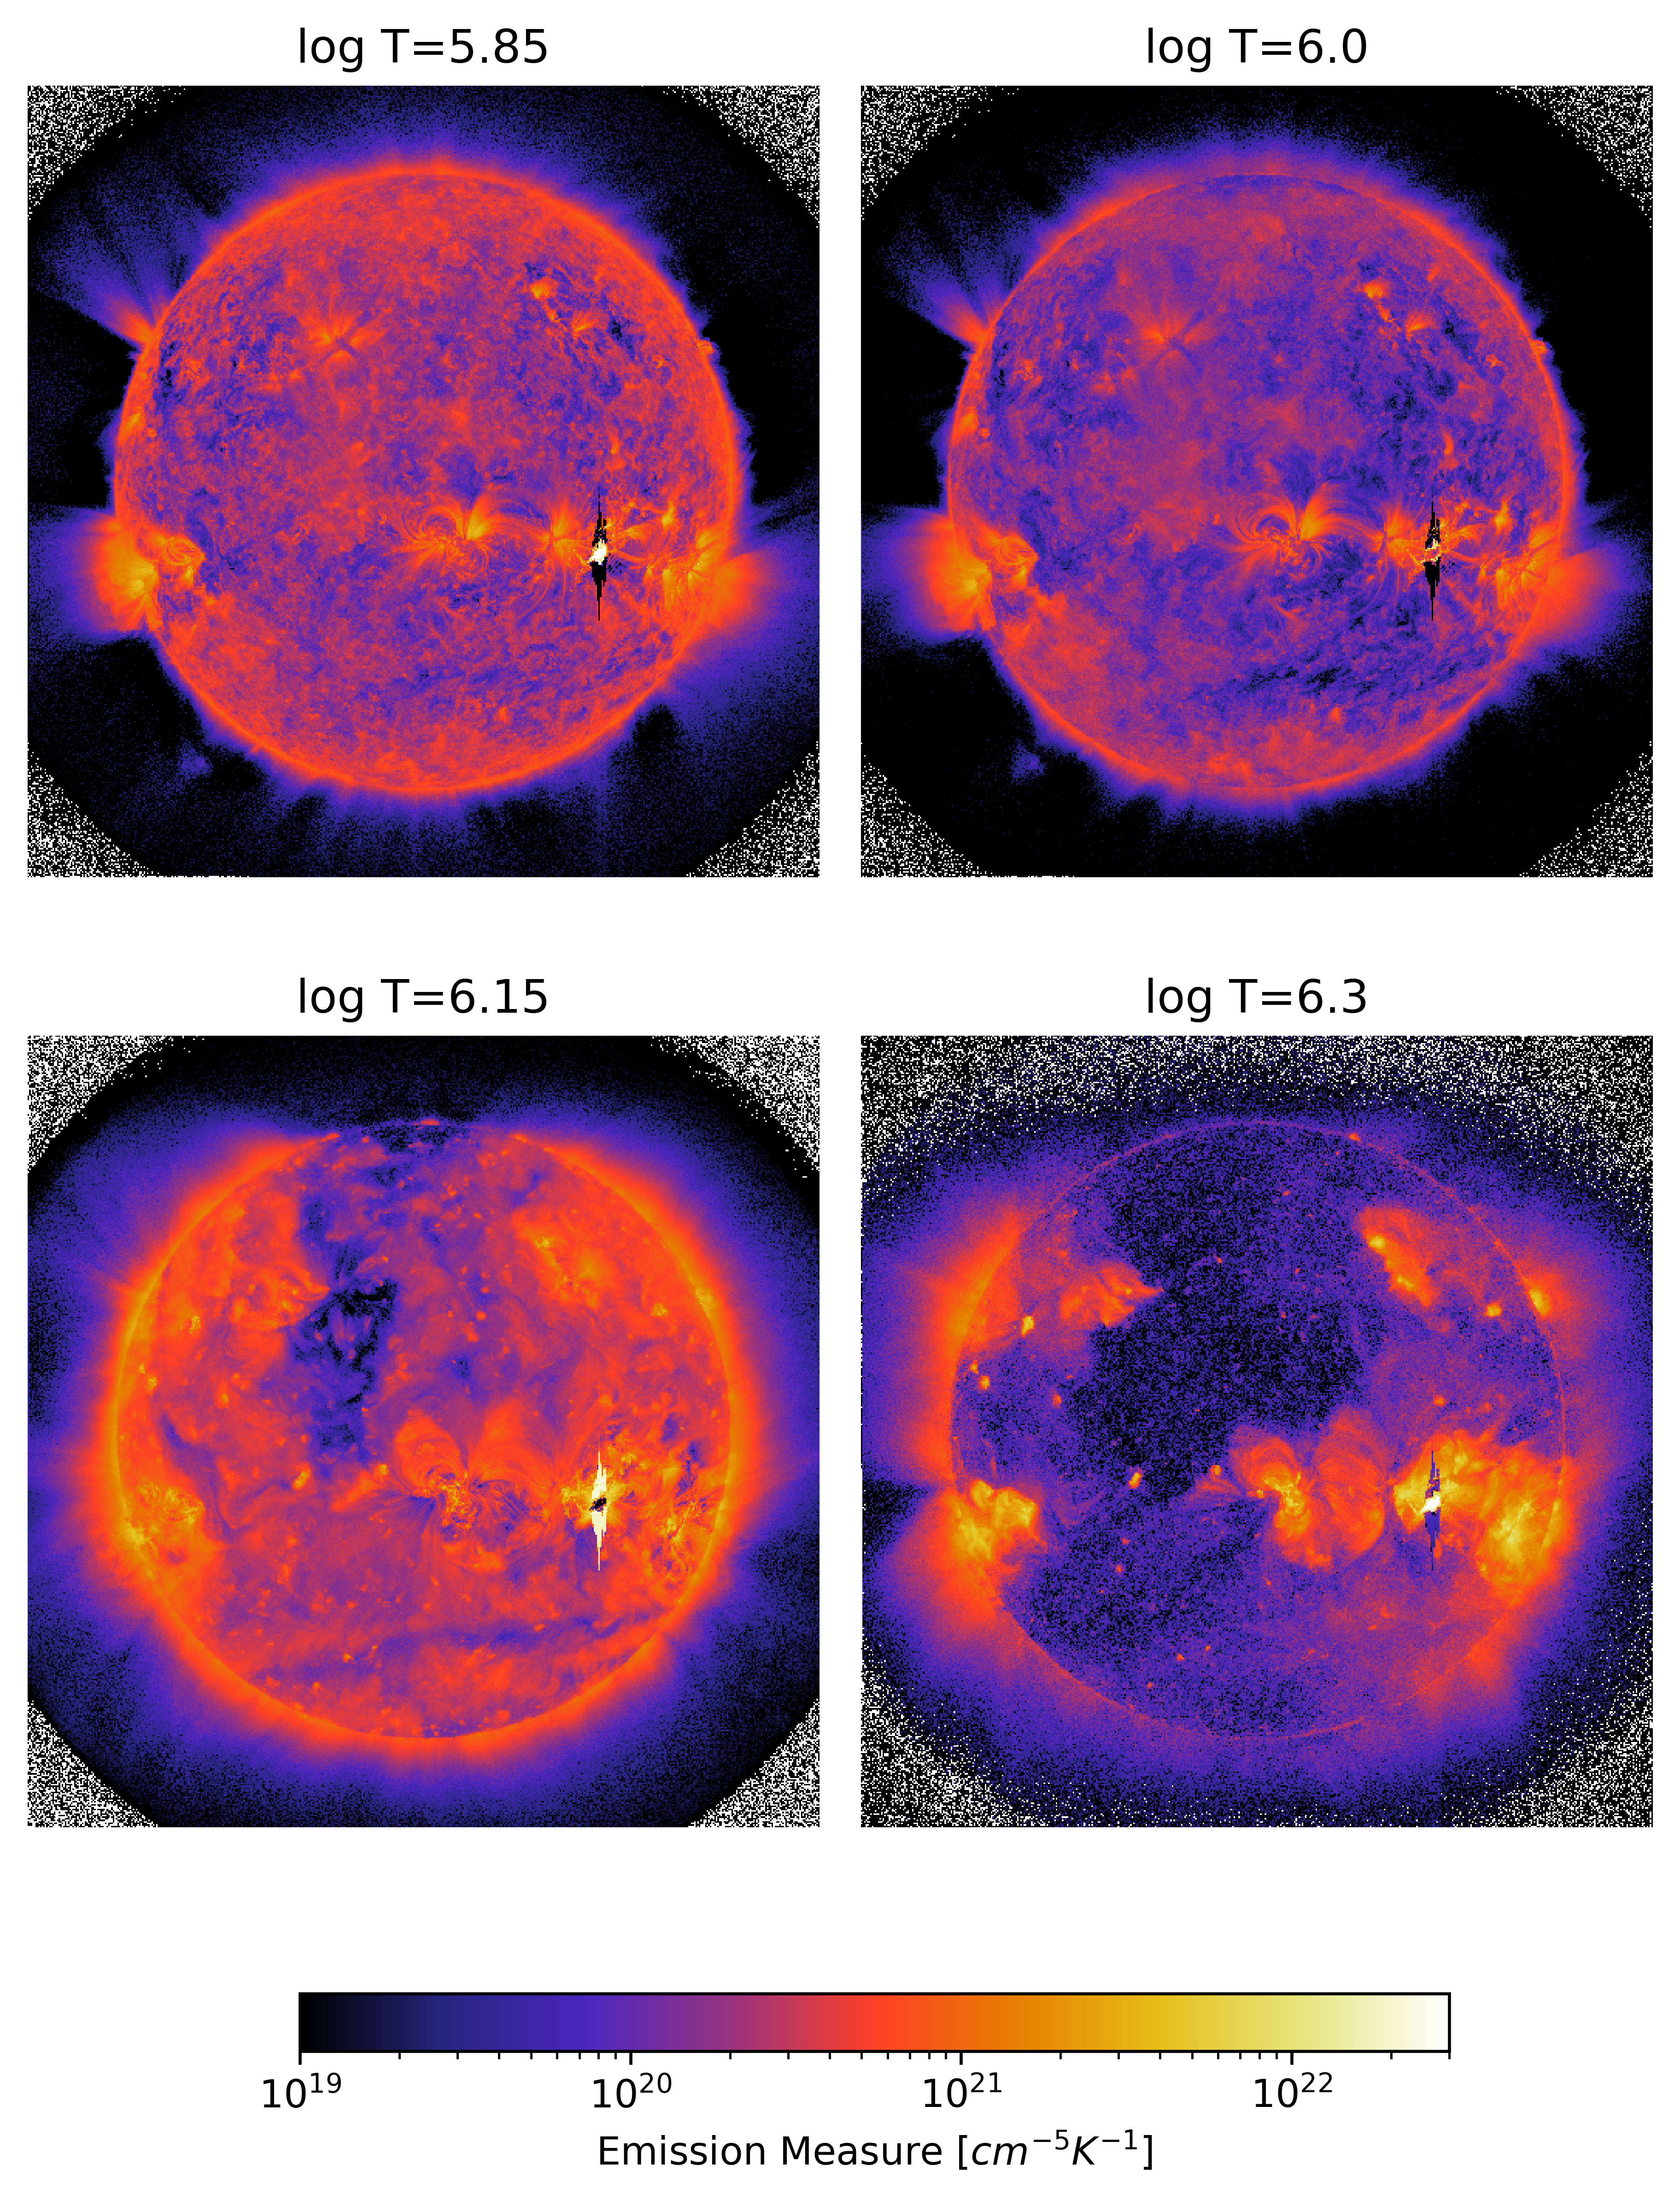
\includegraphics[width=0.5\textwidth]{images/dem_img_aug_4_2011.png}
    \caption[DEM full disk image of Sun]{DEM of Sun during the flaring event on \nth{4} August 2011. The artifacts at the corners of the image is due to the diffraction of light in the telescope of AIA}
    \label{fig:dem_img_aug_4_2011}
\end{figure}

\begin{figure}[h!]
    \centering
    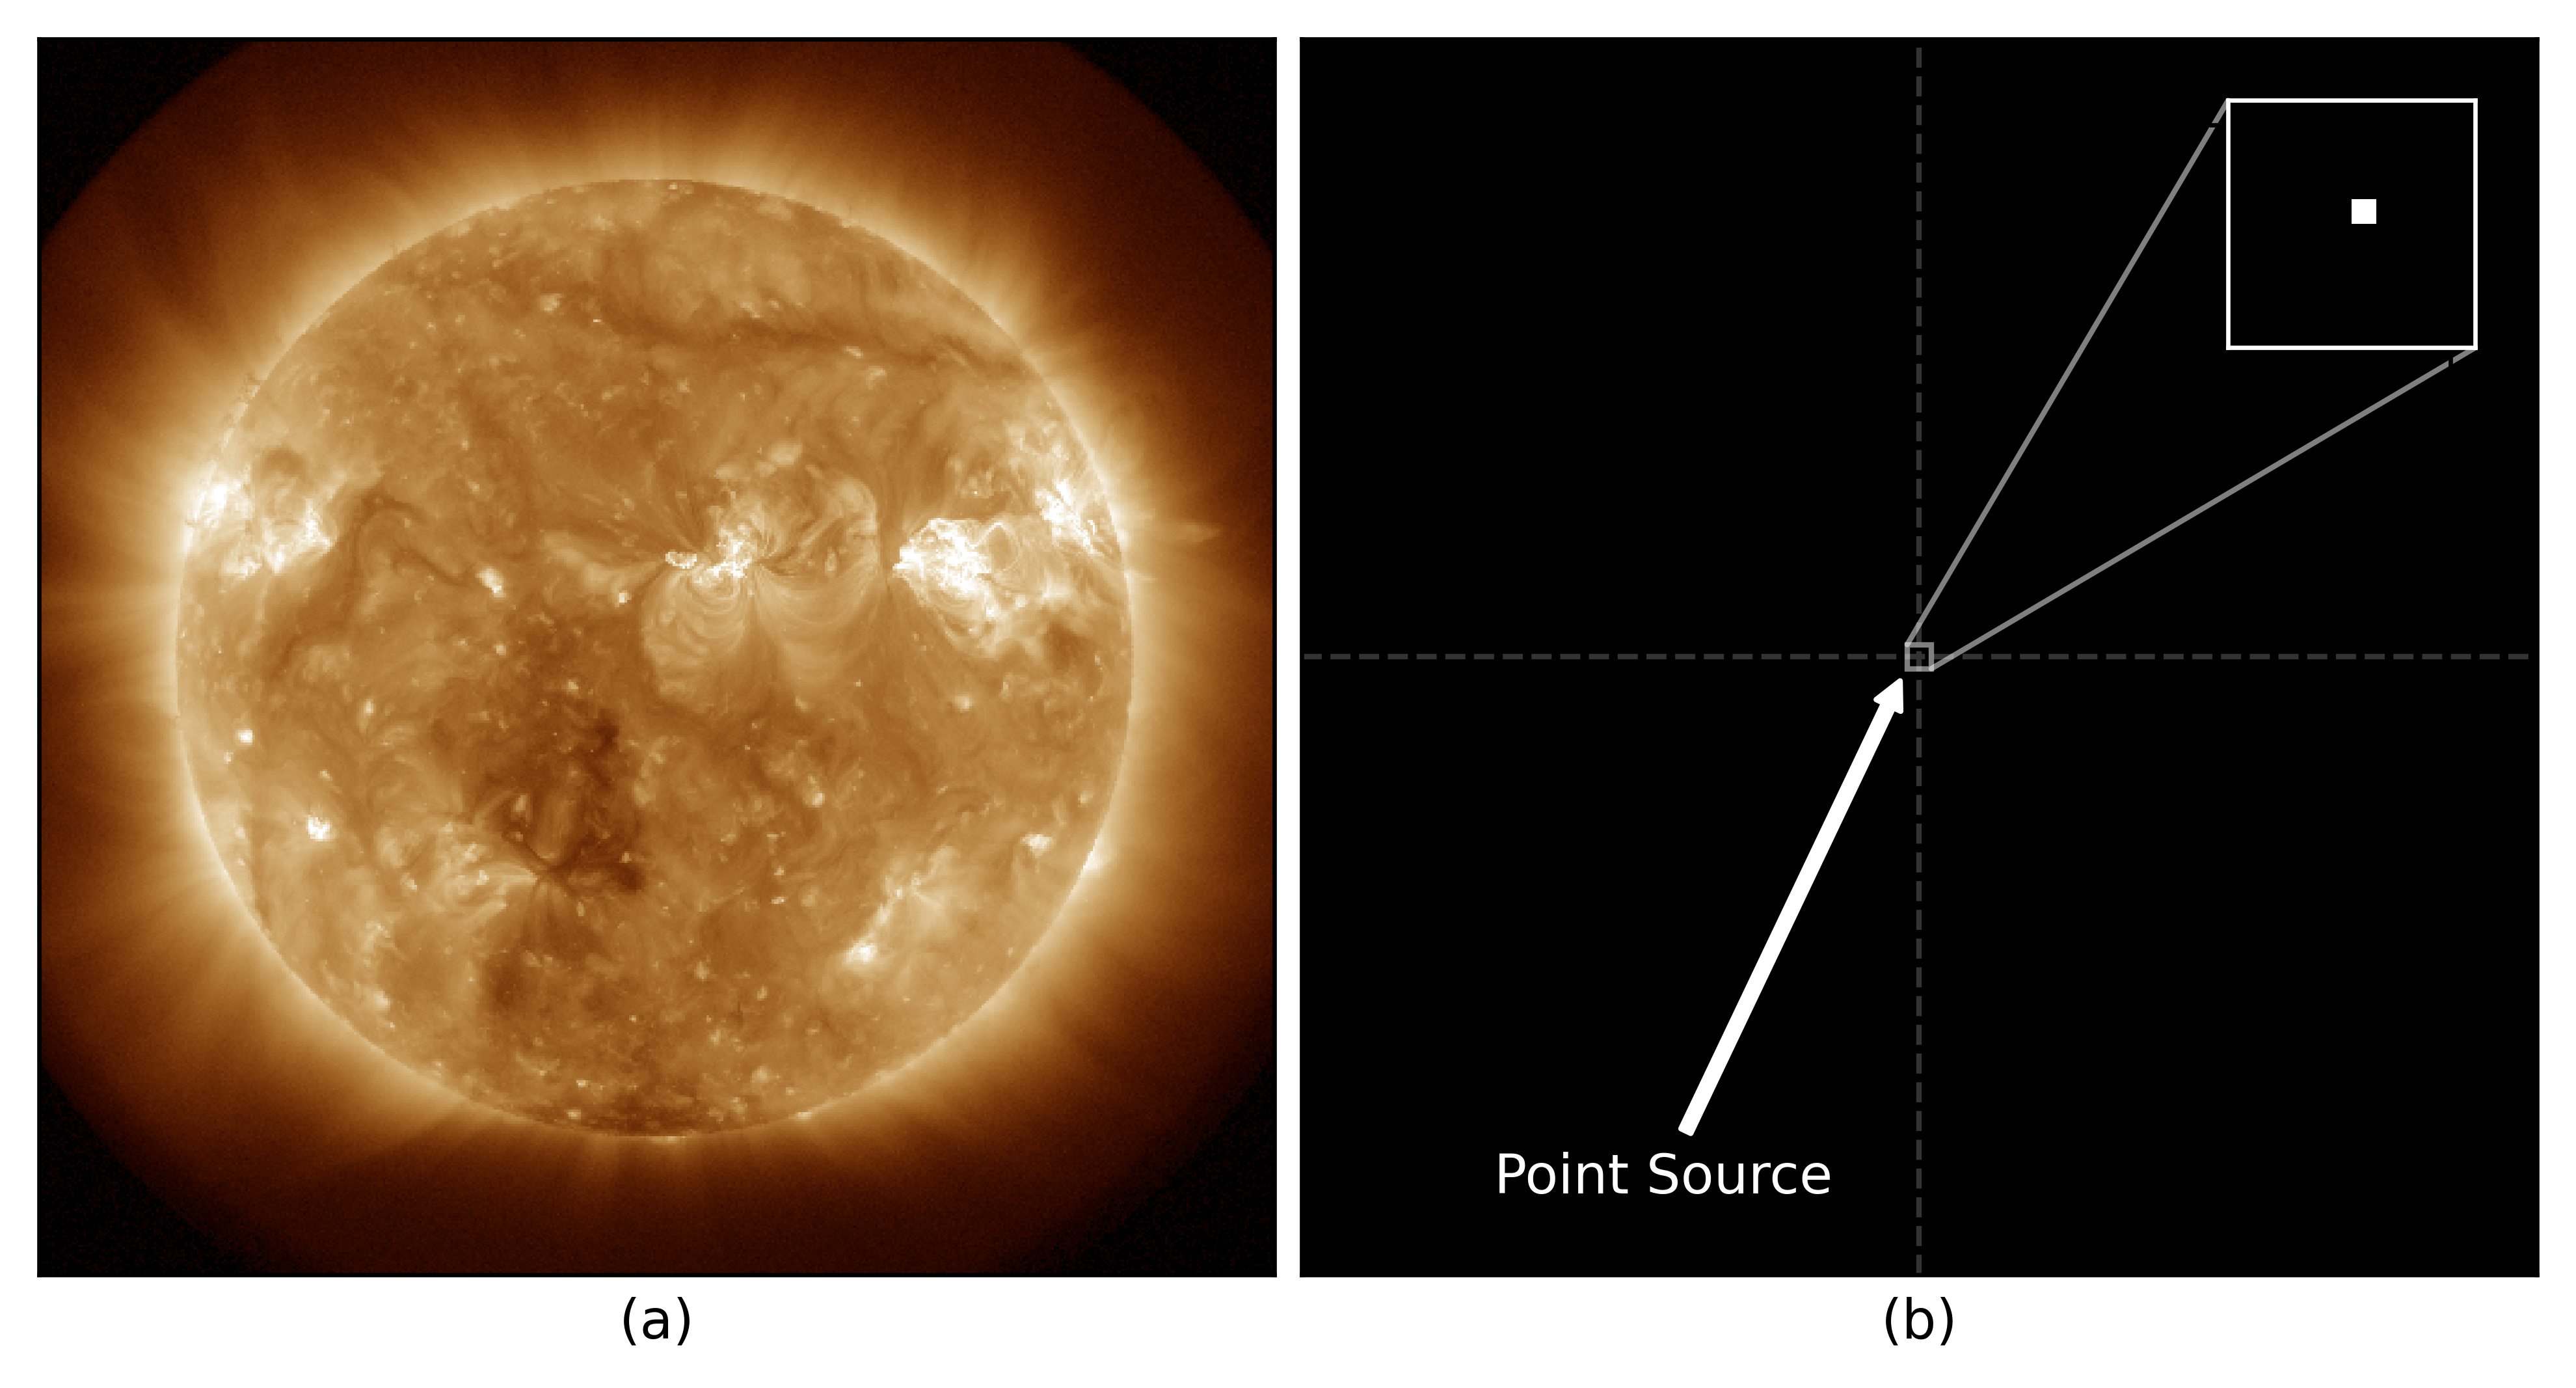
\includegraphics[width=0.95\textwidth]{images/ps_plus_full_disk.png}
    \caption[Full disk and pointified image of Sun]{\textbf{(a)} shows the full disk image of Sun in the 193 $\AA$ channel, \textbf{(b)} shows the image after pointification.}
    \label{fig:ps_plus_full_disk}
\end{figure}

Next step is to generate the point source from the full disk, which we refer to as ``Pointification''. This involves the conversion of the full disk image of Sun to a point source, which mimics a distant star. The original image of 4096 $\times$ 4096 pixels dimension is averaged and new image having 512 $\times$ 512 pixels dimension is created with the pixel value at (256, 256) of the image (midpoint of the image) equal to the calculated average image pixel value. The average values of 4096 $\times$ 4096 pixel image dimension has been considered and not the 512 one so as to not allow the errors due to the resampling of the image affect the average pixel intensity value significantly. \Cref{fig:ps_plus_full_disk} shows the result of pointification procedure. After pointification, DEM profile is reconstructed from these images. These act like DEM profiles of a point source/star.\\

The temperature logT can be grouped into discrete ranges with the corresponding dem solutions being group by averaging. The grouping interval depends on the temperature interval used for the analysis, which in our case is 0.15 K. We have grouped three consecutive temperature intervals (eg: 5.85, 6.0, 6.15). This is called as temperature binning. Binning helps in reducing the impact of noise or uncertainities in the data. By averaging the emission measuresments for each temperature bin, we can smoothen fluctuations and obtain a good estimate of the DEM.

%%% Local Variables:
%%% mode: LaTeX
%%% TeX-master: "main"
%%% End:
